\chapter{Specifikacija programske potpore}
		
	\section{Funkcionalni zahtjevi}
			
			
			\noindent \textbf{Dionici:}
			
			\begin{packed_enum}
				
				\item Klijent teretane
				\begin{packed_enum}
					
					\item registrirani
					\item neregistrirani
					
				\end{packed_enum}
				\item Trener
				\item Voditelj teretane			
				\item Administrator
				\item Razvojni tim
				
			\end{packed_enum}
			
			\noindent \textbf{Aktori i njihovi funkcionalni zahtjevi:}
			
			
			\begin{packed_enum}
				\item  \underbar{Neregistrirani/neprijavljeni korisnik (inicijator) može:}
				
				\begin{packed_enum}
					
					\item pregledati popis svih teretana na platformi
					\item sortirati spomenuti popis prema sljedećim kriterijima: ime teretane, lokacija, trener
					\item otvoriti početnu stranicu svake teretane na kojoj se nalaze osnovne informacije (radno vrijeme, lokacija, cijena
					članarine…)
					\item izraditi administratorski, voditeljski, trenerski ili korisnički račun s namjerom treniranja u teretani za koje je potrebno navesti ime, prezime i email adresu, dok se može, ali ne mora dodati PayPal račun te je za izradu trenerskog korisničkog računa posebno potrebno navesti posebne podatke poput visine i težine
					
					
				\end{packed_enum}
			
				\item  \underbar{Klijent (inicijator) može:}
				
				\begin{packed_enum}
					
					\item pregledavati i sortirati popis registriranih teretana
					\item pregledavati i mijenjati osobne podatke
					\item izbrisati svoj korisnički račun
					\item plaćati članarine u teretanama putem interneta
					\item pregledavati sve izvršene transakcije u kojima su sudjelovali
					\item pregledavati popis teretana u kojima smiju vježbati, odnosno u kojima su platili članarinu
					\item kupovati planove prehrane i vježbanja od trenera
					\item ugovarati privatne ili grupne treninge
					\item voditi i pratiti napredak u vlastitom planu vježbanja
					
				\end{packed_enum}
			
				\item  \underbar{Trener (inicijator) može:}
				
				\begin{packed_enum}
					
					\item pregledavati i sortirati popis registriranih teretana
					\item pregledavati i mijenjati osobne podatke
					\item izbrisati svoj korisnički račun
					\item objavljivati ponude planova treninga i/ili vježbanja
					\item objavljivati i ugovarati termine privatnih i grupnih treninga u teretanama gdje imaju te ovlasti
					\item pregledavati sve izvršene transakcije u kojima su sudjelovali
					\item pregledavati popis teretana u kojima smiju djelovati, odnosno raditi (voditi treninge, planovi prehrane i sl.)
					\item nuditi usluge treniranja teretanama
					
				\end{packed_enum}
		
				\item  \underbar{Voditelj teretane (inicijator) može:}
				
				\begin{packed_enum}
					
					\item pregledavati i sortirati popis registriranih teretana
					\item pregledavati i mijenjati osobne podatke
					\item izbrisati svoj korisnički račun
					\item stvarati nove teretane u sustavu
					\item davati dozvolu drugim voditeljima da vode neke njegove teretane
					\item mijenjati važne informacije o teretanama (radno vrijeme, lokacija i sl.)
					\item dopuštati registriranim trenerima rad u teretanama koje vodi
					\item vidjeti sve izvršene transakcije na aplikaciji unutar vlastite teretane
					
				\end{packed_enum}
	
				\item  \underbar{Administrator (inicijator) može:}
				
				\begin{packed_enum}
					
					\item pregledavati i sortirati popis registriranih teretana
					\item pregledavati i mijenjati osobne podatke
					\item vidjeti sve korisničke račune
					\item izbrisati svoj korisnički račun
					\item stvarati nove i brisati postojeće teretane u sustavu
					\item pregledati sve izvršene transakcije u aplikaciji
					\item davati dozvolu  voditeljima da vode pojedine teretane
					\item mijenjati važne informacije o teretanama (radno vrijeme, lokacija i sl.)
					\item dopuštati registriranim trenerima rad u teretanama
					
				\end{packed_enum}


				\item  \underbar{Baza podataka (sudionik):}
				
				\begin{packed_enum}
					
					\item pohranjuje sve podatke o korisnicima
					\item čuva informacije o ulogama pojedinih korisnika
					\item pohranjuje podatke o svim teretanama, njihovim voditeljima, trenerima i članovima
					\item pohranjuje izvršene transakcije
					
				\end{packed_enum}
		
			\end{packed_enum}
			
			\eject 
			
			
				
			\subsection{Obrasci uporabe}
				
				\textbf{\textit{dio 1. revizije}}
				
				\subsubsection{Opis obrazaca uporabe}
					\textit{Funkcionalne zahtjeve razraditi u obliku obrazaca uporabe. Svaki obrazac je potrebno razraditi prema donjem predlošku. Ukoliko u nekom koraku može doći do odstupanja, potrebno je to odstupanje opisati i po mogućnosti ponuditi rješenje kojim bi se tijek obrasca vratio na osnovni tijek.}\\
					

					\noindent \underbar{\textbf{UC$<$broj obrasca$>$ -$<$ime obrasca$>$}}
					\begin{packed_item}
	
						\item \textbf{Glavni sudionik: }$<$sudionik$>$
						\item  \textbf{Cilj:} $<$cilj$>$
						\item  \textbf{Sudionici:} $<$sudionici$>$
						\item  \textbf{Preduvjet:} $<$preduvjet$>$
						\item  \textbf{Opis osnovnog tijeka:}
						
						\item[] \begin{packed_enum}
	
							\item $<$opis korak jedan$>$
							\item $<$opis korak dva$>$
							\item $<$opis korak tri$>$
							\item $<$opis korak četiri$>$
							\item $<$opis korak pet$>$
						\end{packed_enum}
						
						\item  \textbf{Opis mogućih odstupanja:}
						
						\item[] \begin{packed_item}
	
							\item[2.a] $<$opis mogućeg scenarija odstupanja u koraku 2$>$
							\item[] \begin{packed_enum}
								
								\item $<$opis rješenja mogućeg scenarija korak 1$>$
								\item $<$opis rješenja mogućeg scenarija korak 2$>$
								
							\end{packed_enum}
							\item[2.b] $<$opis mogućeg scenarija odstupanja u koraku 2$>$
							\item[3.a] $<$opis mogućeg scenarija odstupanja  u koraku 3$>$
							
						\end{packed_item}
					\end{packed_item}
				
					
				\subsubsection{Dijagrami obrazaca uporabe}
					
					\textit{Prikazati odnos aktora i obrazaca uporabe odgovarajućim UML dijagramom. Nije nužno nacrtati sve na jednom dijagramu. Modelirati po razinama apstrakcije i skupovima srodnih funkcionalnosti.}
				\eject		
				
			\subsection{Sekvencijski dijagrami}
				
				\textbf{\textit{dio 1. revizije}}\\
				
				\textit{Nacrtati sekvencijske dijagrame koji modeliraju najvažnije dijelove sustava (max. 4 dijagrama). Ukoliko postoji nedoumica oko odabira, razjasniti s asistentom. Uz svaki dijagram napisati detaljni opis dijagrama.}
				
					\subsubsection{Obrazac uporabe UC10 - Učlanjivanje korisnika u određenu teretanu (ili lanac teretana)}
					\textit{}Klijent šalje zahtjev za popis svih teretani te web aplikacija dohvaća popis teretana
                    iz baze podataka te prikazuje klijentu. Klijent potom odabire teretanu te mu se izlistava
                    popis članarina unutar odabrane teretane, tada klijent odabire članarinu koju želi te 
                    ako trenutno nema odabranu članarinu aktivnu dobiva poruku kako je članarina odabrana, 
                    dok ga u suprotnom Web aplikacija preusmjerava natrag na popis članarina za odabrati
                    iz odabrane teretane\\
                    
                    \begin{figure}[H]
			            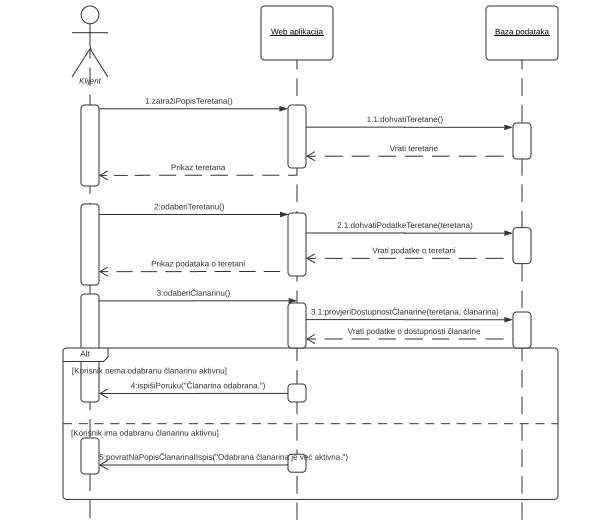
\includegraphics[scale=0.9]{slike/UC10.PNG} %veličina slike u odnosu na originalnu datoteku i pozicija slike
			            \centering
			            \caption{Sekvencijski dijagram za UC10}
			            \label{fig:promjene}
		            \end{figure}
                    
                    
                    \subsubsection{Obrazac uporabe UC13 - Odabir trenerovog programa treniranja ili plana prehrane}
					\textit{}Klijent šalje zahtjev za popis svih trenera te web aplikacija dohvaća popis trenera
                    iz baze podataka te ih sve prikazuje klijentu. Klijent potom odabire trenera. Tada
                    klijent ima opciju odabrati trening ili plan prehrane kod odabranog trenera. U slučaju
                    odabira plana prehrane plan prehrane se pokazuje korisniku. U slučaju odabira treninga,
                    korisnik uz trening odabire i termin treninga. Ako je termin slobodan korisnik dobiva tu
                    informaciju dok u suprotnom dobiva popis slobodnih termina treninga kod odabranog trenera
                    iz kojih potom bira novi termin.\\
                    
                    \begin{figure}[H]
			            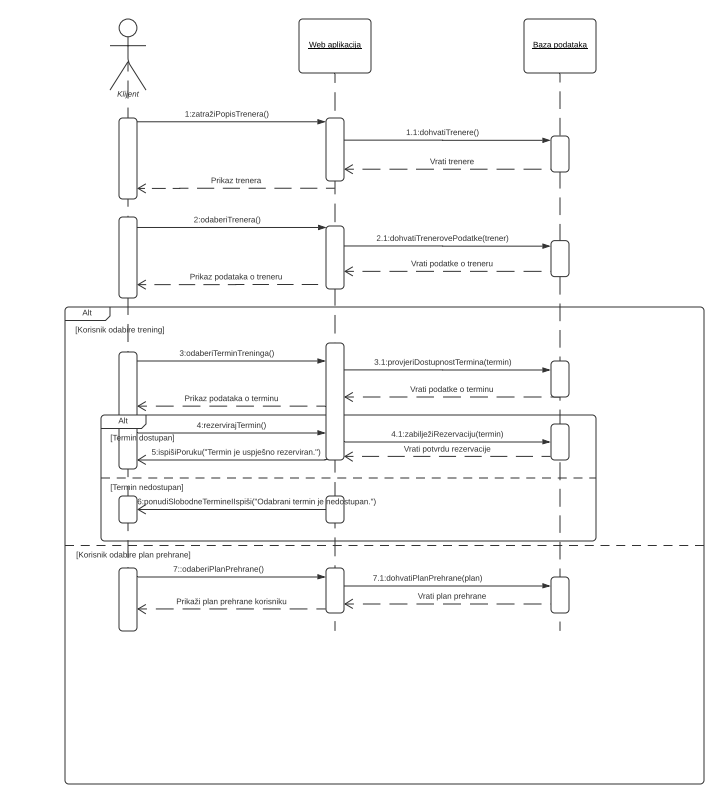
\includegraphics[scale=0.9]{slike/UC13.PNG} %veličina slike u odnosu na originalnu datoteku i pozicija slike
			            \centering
			            \caption{Sekvencijski dijagram za UC13}
			            \label{fig:promjene}
		            \end{figure}
                    
                    
                    \subsubsection{Obrazac uporabe UC15 - Uređivanje trenerove ponude za treninge}
					\textit{}Trener šalje zahtjev za popis svih njegovih programa te web aplikacija dohvaća popis
                    iz baze podataka te ih prikazuje treneru. Trener potom odabire jedan od ponuđenih programa
                    te web aplikacija iz baze podataka povlači informacije o programu te izlistava sve treneru.
                    Trener potom može izmjeniti program te se naknadno ta promjena zabilježava u bazu podataka
                    za buduće izmjene ili potražnje korisnika za tim programom.\\
                    
                    \begin{figure}[H]
			            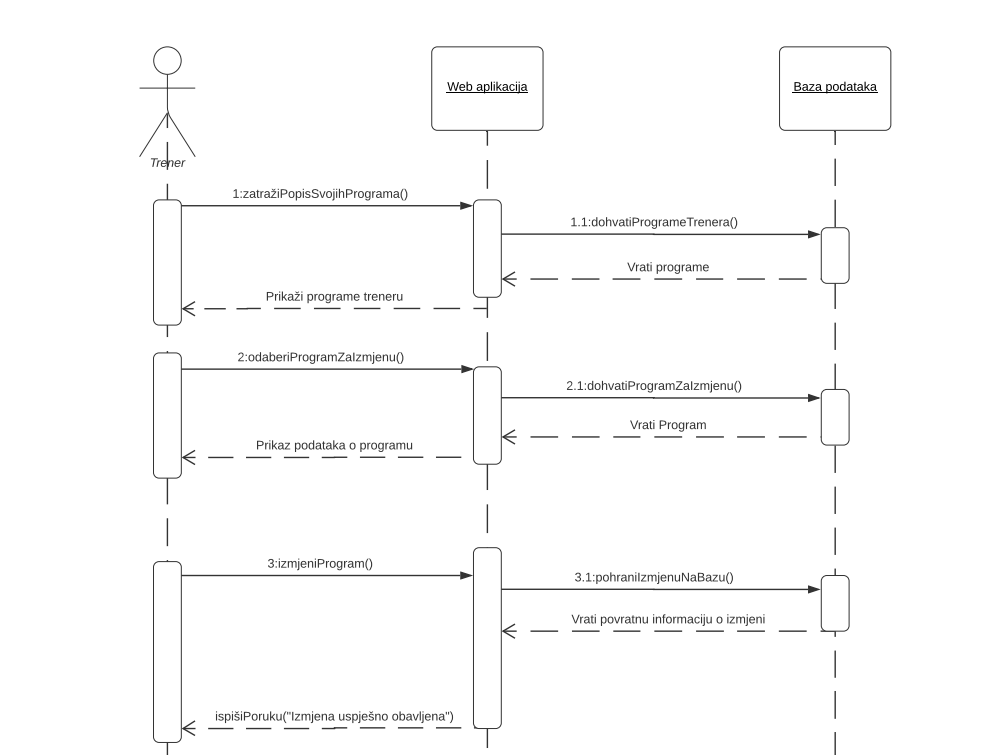
\includegraphics[scale=0.9]{slike/UC15.PNG} %veličina slike u odnosu na originalnu datoteku i pozicija slike
			            \centering
			            \caption{Sekvencijski dijagram za UC15}
			            \label{fig:promjene}
		            \end{figure}
                    
                    
                    \subsubsection{Obrazac uporabe UC16 - Dozvola za rad trenera u teretani}
					\textit{}Trener šalje zahtjev za popis svih teretani te web aplikacija dohvaća popis
                    iz baze podataka te ih prikazuje treneru. Trener potom odabire teretanu za 
                    koju je zainteresiran, a podaci o teretani se ponovo dohvaćaju iz baze podataka.
                    Tada trener šalje zahtjev za rad u teretanu, a web aplikacija u bazi provjerava
                    radi li već trener u odabranoj teretani. U slučaju da ne radi u odabranoj teretani
                    dobiva poruku kako je zahtjev uspješno zaprimljen te zahtjev čeka odobrenje voditelja
                    teretane, a u slučaju da trener ondje već radi dobiva poruku koja ga o tome obavještava.\\
                    
                    \begin{figure}[H]
			            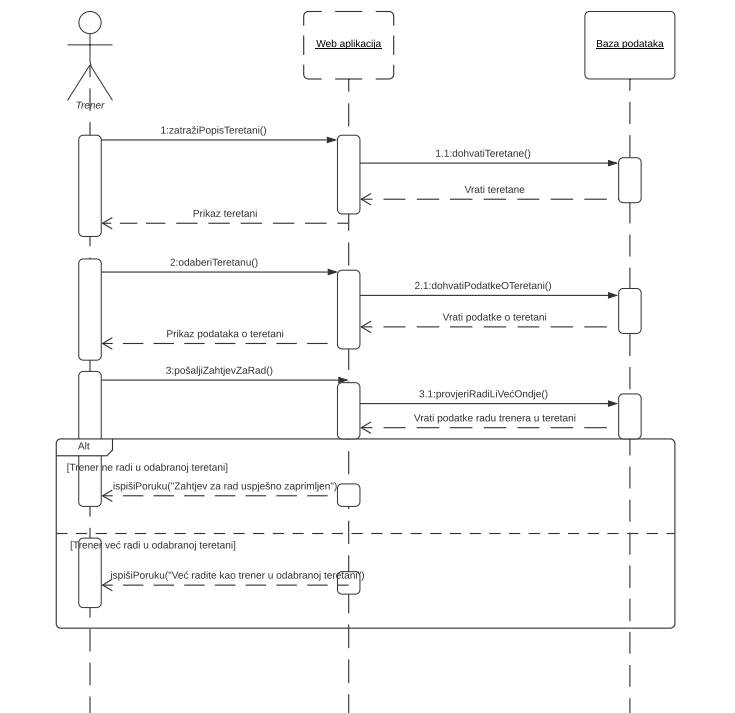
\includegraphics[scale=0.9]{slike/UC16.PNG} %veličina slike u odnosu na originalnu datoteku i pozicija slike
			            \centering
			            \caption{Sekvencijski dijagram za UC16}
			            \label{fig:promjene}
		            \end{figure}
                    
				
				
				\eject
	            
	            
	            
		\section{Ostali zahtjevi}
		
			\textbf{\textit{dio 1. revizije}}\\
		 
			 \textit{Nefunkcionalni zahtjevi i zahtjevi domene primjene dopunjuju funkcionalne zahtjeve. Oni opisuju \textbf{kako se sustav treba ponašati} i koja \textbf{ograničenja} treba poštivati (performanse, korisničko iskustvo, pouzdanost, standardi kvalitete, sigurnost...). Primjeri takvih zahtjeva u Vašem projektu mogu biti: podržani jezici korisničkog sučelja, vrijeme odziva, najveći mogući podržani broj korisnika, podržane web/mobilne platforme, razina zaštite (protokoli komunikacije, kriptiranje...)... Svaki takav zahtjev potrebno je navesti u jednoj ili dvije rečenice.}
			 
			 
			 
	